\documentclass[useAMS,usenatbib]{mn2e_x}
%%%% Various options for document class.
%\usepackage{psfig,morefloats,url}
%use preprint2 for 2 columns paper.

%% declare any packages used
\usepackage{graphicx}
\usepackage{natbib}
\usepackage{graphicx}
\usepackage{color}
\usepackage{pdfpages}
\usepackage{appendix}
\usepackage{subfigure}
\usepackage{url}
\usepackage{amsmath}
%\usepackage{pngfig}
%\usepackage[dvips]{color}mak
%\usepackage{aabib}


%\marginparwidth = 25pt
\citestyle{aa}
\addtolength{\topmargin}{-.5in}
%\addtolength{\bottommargin}{-1in}
%% This command added as margins are wrong in mn2e, it appears. 
%% Not needed for other classes
\usepackage{float}



%%%%%%%%%%%%%%%%%%%%%%%%%%%%%%%%%%%%%%

\begin{document}
%% define bibstyle and other definitions
\bibliographystyle{aabib}
%% renew commands
%%\renewcommand{\labelitemi}{$.$}

%% Codes
\def\py{\textsc{Python}}
\def\tar{\textsc{Tardis}}
\def\cld{\textsc{Cloudy}}
\def\agn{\textsc{Agnspec}}


%% Lines and ions
\def\civ{C~\textsc{iv}}
\def\nv{N~\textsc{v}}
\def\hei{He~\textsc{i}}
\def\heii{He~\textsc{ii}}
\def\mg{Mg~\textsc{ii}}
\def\al{Al~\textsc{iii}}
\def\heii{He~\textsc{ii}}
\def\ovi{O~\textsc{vi}}
\def\la{Ly~$\alpha$}
\def\ha{H~$\alpha$}
\def\hb{H~$\beta$}



%% Journal definitions
\def\araa{ARAA}
\def\nat{Nature}
\def\apjl{ApJ Letters}
\def\aapr{AAPR}
\def\ssr{SSR}
\def\apj{ApJ}
\def\apjs{ApJs}
\def\pasp{PASP}
\def\aap{A\&A}
\def\mnras{MNRAS}
\def\aj{AJ}
\def\rmxaa{RMXAA}
\def\aaps{A\&As}
\def\LA{Lyman\thinspace$\alpha$}

\newcommand{\EXPN}[2]{\mbox{$#1\times 10^{#2}$}}
\newcommand{\EXPU}[3]{\mbox{\rm $#1 \times 10^{#2} \rm\:#3$}}  % exponent with units
\newcommand{\POW}[2]{\mbox{$\rm10^{#1}\rm\:#2$}}
\def\LUM{\:{\rm erg\:s^{-1}}}
\def\FLUX{\:{\rm erg\:cm^{-2}\:s^{-1}}}
\def\OIGS{\:{\rm erg\:cm^{-2}\:s^{-1}\:\AA^{-1}}}

%%%%%%%%%%%%%%%%%%%%%%%%%%%%%%%%%%%%%%
%
%          TITLE AND AUTHORS
%
%%%%%%%%%%%%%%%%%%%%%%%%%%%%%%%%%%%%%%%

\title
{
% Modelling quasar outflows:
% clumpy winds and broad emission lines
Testing Quasar Unification with Clumpy Wind Models
%Unifying quasars with clumpy wind models
}


%\author[Matthews et al.]
\author[Matthews et al.]{
\parbox[t]{\textwidth}{
James~H.~Matthews$^1$\thanks{jm8g08@soton.ac.uk}, Christian~Knigge$^1$,
Nick~Higginbottom$^1$, Knox~S.~Long$^2$, Stuart~A.~Sim$^3$ and Sam~W.~Mangham$^1$
}
\medskip  
\\$^1$School of Physics and Astronomy, University of Southampton, Highfield, Southampton, SO17 1BJ, United Kingdom
\\$^2$Space Telescope Science Institute, 3700 San Martin Drive, Baltimore, MD, 21218
\\$^3$School of Mathematics and Physics, Queens University Belfast, University Road, Belfast, BT7 1NN, Northern Ireland, UK
}





\date{\today}
%\\
%Supervisor: Prof. Christian Knigge\\
%{\sl School of Physics \& Astronomy, University of Southampton,
%  Southampton, SO17 1BJ, UK}}


%%%%%%%%%%%%%%%%%%%%%%%%%%%%%%%%%%%%%%
%
%          ABSTRACT
%
%%%%%%%%%%%%%%%%%%%%%%%%%%%%%%%%%%%%%%%


\begin{abstract} 
% Broad absorption lines (BALs) in the ultraviolet 
% are seen in $\sim20\%$ of quasi-stellar objects (QSOs). 
% Blue-shifted broad absorption lines (BALs) are the most direct evidence of 
% accretion disc `winds' in such systems; mass loaded outflows
% emanating from the disc that may be driven by line forces or
% magnetic processes. 
% Various unification schemes for
% quasars and luminous active galactic nuclei (AGN) have proposed
% that the broad emission line region is roughly cospatial
% with broad absorption line (BAL) gas and much of the phenomenology of luminous AGN
% can be explained by a simple geometrical picture involving an accretion
% disc and associated outflow. Here, we test this paradigm by 
% utilising our state-of-the-art radiative transfer code to produce synthetic spectra
% from simple biconical disc wind models. 
% In particular, we expand on our previous 
% work in which a benchmark model for BAL quasars was produced. 
% We have conducted a limited parameter search with the aim of unifying quasar phenomenology,
% and arrive at an improved model. The grid is now publicly available.
% We find that a simple treatment of clumping (`microclumping') 
% allows for a more realistic X-ray luminosity in the model by lowering the 
% ionization parameter. We examine the X-ray properties of this new model
% and find good agreement with existing X-ray samples of AGN and QSOs.
% We find that the dense, X-ray heated wind 
% produces strong H recombination and collisionally excited resonance 
% line emission to emerge at the low inclination angles, 
% which represent quasars within this unification scenario.
% % We also treat Hydrogen using a `macro-atom' approach in order to 
% % examine the effect of recombination on Hydrogen emission lines, and
% % this results in significant line emission in Lyman~$\alpha$ and the Balmer series.
% However, we are unable to reproduce the remarkably similar of line-to-continuum
% ratios between BAL and non-BAL quasar composites.
% This is due to a fundamental constraint arising
% from the anisotropy of emission from a classical thin disc. 
% We briefly explore the effect of relativistic beaming, gravitational redshift and 
% light bending on the angular distribution of disc continuum emission. 
% We find that these general relativistic effects do cause the disc to
% emit slightly more isotropically, but this is not yet sufficient to produce a
% self-consistent model. We discuss wind reprocessing as a potential solution.
% Overall, our work suggests that geometric unification
% involving an accretion disc wind is a promising scenario, but our results 
% pose a number of difficult challenges to such a model.
% Determining the true geometry of ADWs and uncovering the true disc spectral 
% (and angular) energy distribution are key next stpng if we are to build up a 
% holistic picture of the quasar population.
Various unification schemes have been proposed to interpret the complex phenomenology 
of quasars and luminous active galactic nuclei (AGN) in terms of  a simple axisymmetric 
picture involving a central black hole, an accretion disc and an associated outflow.
Here, we continue our tests of  this paradigm by comparing quasar spectra to 
synthetic spectra of simple biconical disc wind models, produced with our state-of-the-art 
Monte Carlo radiative transfer and photoionization code PYTHON.  Previously, we have shown that we could produce synthetic spectra resembling those of observed AGN for plausible wind models, but only if the X-ray luminosity was limited to about  10$^{43}$ erg s$^{-1}$.  Here , we investigate the  degree to which  clumping of the outflow allows us to 
produce synthetic spectra in the rest-frame UV that have the characteristics of quasars with X-ray luminosities as large as 10$^{45}$ erg s$^{-1}$. 
We conclude, perhaps not surprisingly,  that clumping does maintain the ionization state of the wind necessary for strong BAL features in the rest-frame UV at more realistic X-ray luminosities. We examine the X-ray properties of these simple clumped models
and find good agreement with existing X-ray samples of AGN and quasars.
In addition, the dense, X-ray heated wind produces strong recombination and collisionally 
excited line emission in, e.g., \civ\ and \la, to emerge at the low inclination, 
`Type 1 quasar-like' angles. At the highest inclinations, the synthetic spectra possess prominent \mg\ and \al\ BALs, the absorption features seen in LoBAL quasars. 
Despite these successes, we are unable to reproduce 
the remarkably uniform emission line properties 
seen in BAL and non-BAL quasar composites, as we find a marked increase
in emission line equivalent widths at high inclination `BALQSO-like' angles. 
This is due to a fundamental constraint arising
from the anisotropy of emission from a classical thin disc. 
Overall, our work suggests that geometric unification
involving an accretion disc wind is a promising scenario, but our results 
pose a number of difficult challenges to models in which an equatorial outflow
rises from a limb-darkened, foreshortened accretion disc.
% {\bf There is confusion in the abstract, at least, in what is the model and what is the synthetic spectra, as well as whether there is one model or many models.  We need to try to be clear.  The model should be a clumped biconical outflow.  There are then particular instantiations of the model. And then there are synthetic spectra}
\end{abstract}

%\begin{keywords}
%AGN: outflows
%\end{keywords}

\maketitle

%%%%%%%%%%%%%%%%%%%%%%%%%%%%%%%%%%%%%%
%
%          INTRODUCTION
%
%%%%%%%%%%%%%%%%%%%%%%%%%%%%%%%%%%%%%%%

\section{Introduction}

The spectra of 
quasars and luminous active galactic nuclei (AGN) 
typically exhibit a series of strong emission lines
with an underlying blue continuum - the so-called {\sl `big blue bump'} (BBB). 
The BBB is often attributed to emission from a 
geometrically thin, optically thick accretion disc surrounding the central black hole, similar
to that described by \cite{shakurasunyaev1973}.
% {\bf Note: the first half of this paragraph and the second do not follow from one another.  
% The first half is about spectra the second about outflows and the connection to spectra is not made until the next paragrph.  
% This needs fixing. JM: Knox, I like this structure...I start with inflow, then move to outflow.}
In addition to the {\em inflowing} accreting material, 
{\em outflows} are ubiquitous in AGN
and quasars \citep{kellerman1989,ganguly2008}. These outflows can take the form of 
highly collimated radio jets \citep[e.g.][]{hazard1963,potash1980,perley1984,marscher2006}, 
or mass-loaded `winds' emanating from the accretion disc 
\citep{weymann1991,turnermiller2009}. 
Outflows in AGN offer a 
potential feedback mechanism through which the central source can 
affect its environment \citep{king2003,king2005,fabian2012}
-- feedback that is required in models of galaxy evolution \citep{springel2005}
and may explain the `$M-\sigma$' relation \citep{silkrees1998,haring2004}.

Perhaps the clearest evidence of outflows in AGN is  
the blueshifted ($\sim 0.1c$) broad absorption lines (BALs) in the 
ultraviolet seen in approximately $20\%$ of quasars
\citep{weymann1991, reichard2003, knigge2008, turnermiller2009, allen2011}.
The simplest explanation for the incidence of 
BAL quasars (BALQSOs) is in terms of an accretion disc wind. 
According to this paradigm, a biconical wind rises from 
the accretion disc and the BALQSO fraction is associated with
the covering factor of the outflow. 
Polarisation studies expect the wind to be roughly equatorial
\citep{goodrich1995, cohen1995}, although there is also evidence
for polar BAL outflows  in radio-loud (RL) sources \citep{zhou2006}.
% although this geometry is contradicted
% by more recent studies of radio spectral indices \citep{dipompeo2012}.

Due to their ubiquitous nature,
disc winds offer a natural explanation for the
diverse phenemonology of luminous AGN and quasars \citep[e.g.][]{MCGV95, elvis2000}. 
Depending on viewing angle, an observer 
may see a BALQSO or normal `Type 1' quasar.
Within this {\em geoemtric unification} framework, the broad-line region (BLR) can 
correspond either to the dense wind base or clumps embedded
in the outflow. Indeed, \cite{elitzur2014} show that a disc-wind BLR scenario
naturally explains the emission line evolution of AGN.
A biconical wind model can also readily explain the various sub-classifications of BALQSOs: 
HiBALQSOs, which only exhibit high ionization line absorption; LoBALQSOs, which also show
absorption in lower ionization state species such as \mg\ and \al; and
FeLoBALQSOs, which show further absorption in Fe~\textsc{ii} and \textsc{iii}.
In unified geometric models, this is generally attributed to ionization stratification
of the outflow \citep[e.g.][]{elvis2000}.

% As well as acting as a source of photoionized plasma, a 
% As well as imprinting clear line absorption and emission
% features, disc winds may also have a profound effect on the structure and 
% emergent {\em continuum} of the accretion disc itself.
% Mass-loss will alter the accretion rate and resultant 
% temperature of the accretion disc, possibly explaining some 
% of the features typically seen in luminous AGN \citep{knigge1999,laordavis2014}.
% There have been numerous difficulties when confronting 
% theoretical accretion disc models with observations 
% \citep[see e.g.][]{blaes1998}. However, AGN spectral energy distributions (SEDs) can now, 
% in general, be fitted well with accretion disc models
% when the effects of general relativity (GR), Comptonisation
% and mass-loss are included \citep{capellupo2015}. Mass-loss therefore appears to be 
% critical if an accretion disc model is to successfully fit AGN SEDs, 
% particular in the UV region of the spectrum.

%{\bf ksl: I don't see what this paragraph has to do with our problem, which we need to clearly explain} Despite the clear importance of ADWs in understanding AGN SEDs and accretion physics,
Despite the clear importance of disc winds in shaping quasar and AGN spectra,  
much of the underlying outflow physics remains highly uncertain. 
Several possible driving mechanisms have been proposed, including
thermal pressure \citep{weymann1982, begelman1991}, magnetocentrifugal forces 
\citep{blandfordpayne,pelletier_pudritz} and 
radiation pressure on spectral lines \citep[`line-driving';][]{lucysolomon1970,shlosman1985,MCGV95}.
Of these, line-driving is possibly the most attractive, as
strong absorption lines are already seen in BALQSOs and the X-ray spectra of AGN 
\citep{reeves2003,poundsreeves2009,tombesi2010a}.
% The presence of line-locked features \citep{bowler2014} 
% and the `ghost of \la' (Arav et al. 1996; Arav 1996; North 2006; but see 
% also Cottis et al. 2010) \nocite{arav1995, arav1996, north2006,cottis2010}
% in the spectra of some BALQSOs also gives clearer evidence that line-driving is
% at least partially contributing to the acceleration of the wind.
The efficiency of line-driving is crucially dependent on the ionization state 
of the outflowing plasma, meaning that it is difficult to prevent 
the wind becoming over-ionized and `failing' in the presence of strong X-rays. 
\cite{MCGV95} proposed a potential solution: 
a region of `hitchhiking gas' that could shield the wind from the central X-ray source. 
% Hydrodynamic simulations of line-driven disc winds also found a shielding region
% was required to maintain the correct ionization state \citep{PSK2000,PK04}. 
% However, \cite{sim2010_hydro} and \cite{H14} showed that including multiple scattering means the ionizing radiation field could still reach the previously shielded regions 
% in those particular models.
An additional or alternative solution is that the wind is clumped \citep[e.g.][]{hamann2013}
possibly on multiple scale lengths. Local density enhancements could lower the 
ionization parameter of the plasma while still maintaining the same mass-loss 
rate and column density. 

Evidence for dense substructures in AGN winds is widespread.
BALQSOs show complex absorption line profiles \citep{ganguly2006, simonhamann2010}
and exhibit variability in these profile shapes \citep{capellupo2011,capellupo2012,capellupo2014}.
AGN generally show variability in X-ray absorption components \citep[e.g.][]{risaliti2002}
and many models for the BLR consist of clumps embedded in an outflow 
\citep{krolik1981, emmering1992, dekool1995, cassidyraine1996}.
Clumping can be caused by magnetic confinement \citep{dekool1995},
or the instabilities inherent to line-driven winds 
\citep{lucysolomon1970,macgregor1979,carlberg1980,owockirybicki1984,owockirybicki1985}.
Additionally, clumping is required to explain the electron scattering wings of emission lines formed
in line-driven hot star winds \citep{hillier1991eswingsmodel}. Complex substructures 
are also produced in simulations of line-driven 
outflows in AGN, although on very different scales to line-driven instabilities 
\citep{PSK2000,PK04,progakurosawa2010,proga2014}.  
% {\bf KSL: I do not believe the AGN simulations have the resolution to produce clumping on the scale of hot star winds.
% JM: that's why I mention scales, although I can specifically mention resolution if we
% want.}
Nevertheless, clumpy winds offer an observationally motivated and theoretically 
predicted way to lower the ionization state of a plasma, possibly in tandem
with a shielding scenario. 

We have been engaged in a project to determine whether it is possible to simulate the properties of the spectra of AGN, including BALQSOs, using simple kinematic prescriptions for biconical disc winds using a Monte Carlo radiative transfer (MCRT) code that calculates the ionization structure of the wind and simulates the spectra from such a system \citep[][hereafter H13]{simlong2008,sim2010,higginbottom2013}.  The results have been encouraging in the sense that in H13, we showed we could produce simulated spectra that resembled that of BALQSOs, as long as the luminosity of the X-ray source was relatively low, of order \POW{43}{\LUM} and the mass loss rate was relatively high, of order the mass accretion rate.  However, at higher X-ray luminosities, the wind was so ionized that UV absorption lines were not produced.  In addition, and in part due to limitations in our radiative transfer code, the model failed to produce spectra with strong emission lines at any inclination angle.  

Here we attempt to address both of these issues, by introducing clumping into our model and a more complete treatment of H and He into our radiative transfer calculations.   The remainder of this paper is organized as follows:
% There has been some success using simple kinematic prescriptions for biconical disc winds to model  AGN and quasar outflows \citep[][hereafter H13]{simlong2008,sim2010,higginbottom2013}.  H13 successfully produced a benchmark model for BALQSOs. However, the model had two key drawbacks. First, an unrealistically low X-ray luminosity was required in order to prevent over-ionization of the outflow. Second, the model failed to produce the strong emission lines  required at low inclinations in a unified model. In this paper, we attempt to address these issues, and test the disc wind  unification model using Monte Carlo radiative transfer (MCRT) and photoionization  calculations. The paper is organised as follows.
In section 2, we describe some of the important photoionization 
and MCRT aspects of the code. We then outline the model in section 3, including 
a description of our clumping implementation and success criteria. 
Section 4 contains the results from a clumped model, which we discuss results
in comparison to observational data. Finally, we summarise our findings in section 5.


%%%%%%%%%%%%%%%%%%%%%%%%%%%%%%%%%%%%%%%%%%%%%%%%%

% MCRT

%%%%%%%%%%%%%%%%%%%%%%%%%%%%%%%%%%%%%%%%%%%%%%%%%

\section{Ionization and Radiative Transfer}

For this study, we use the MCRT code \py 
\footnote{Named {\sl c. 1995}, predating the inexorable rise of a certain progamming language.} we have developed to carry out our 
radiative transfer and photoionization simulations in non-local-thermodynamic-equilibrium 
(non-LTE). The code can be used to model a variety of
disc-wind systems; it has been used with application to accreting white dwarfs 
(Long \& Knigge 2002, hereafter LK02; Noebauer et al. 2010; 
Matthews et al. 2015, hereafter M15), young-stellar objects 
\citep{simmacro2005} and quasars/AGN (H13, H14).\nocite{noebauer, M15, LK02}  

The code operates as follows:   This outflow is discretized into $n_x \times n_z$ cells in a 2.5D
cylindrical geometry with azimuthal symmetry. From some initial conditions in each cell, the code first calculates the ionization structure of the wind in a series of iterations.  Each iteration in an ``ionization cycle'' consists of generating photons, actually photon packets, from an accretion disc
and central object, and calculating how these photon bundles scatter through the wind (eventually escaping the outflow or hitting the disk). Then updating the ionization structure based on the properties of the radiation field in each cell, and the process is repeated.   Once the ionization structure has converged, the ionization structure is held fixed, and  synthetic spectra are generated at specific inclination angles in a series of "spectral cycles". LK02 provide a more detailed  description of the original code; various improvements have been made since then and are described by \cite{simmacro2005}, H13 and M15.  
%A full description of the code will be published elsewhere; 
We focus here on the specific changes made for this study intended to improve the ionization calculation of H and He
and to allow for clumping in the wind.
%These studies contain extensive detail on the code,  so we only briefly describe the key elements of the global ionization calculation and other important aspects.


\subsection{Line transfer}

Our approach to line transfer is based upon the macro-atom implementation developed by 
\cite{lucy2002, lucy2003}, in which the energy flows through the system are described in 
terms of indivisible energy quanta of radiant or kinetic energy 
(`$r-$packets' and `$k-$packets' respectively; see also section~\ref{sec:photon_sources}). 
In our case, for reasons of computational efficiency, we adopt the  hybrid macro-atom scheme 
described by M15.
%(an improvement over that used by H14 for our earlier quasar study), 
In this scheme, the energy packets interact with either two-level `simple ions' 
or full `macro-atoms'. This allows one to treat non-LTE line transfer in radiative equilibrium, which assumes both statistical equilibrium and that 
radiative heating balances radiative cooling.
% {\bf KSL: what does "in radiative equilibrium" here mean? 
% JM: Defined.}
without approximation for elements that are identified as 
full macro-atoms, while maintaining the fast `two-level' 
treatment of resonance lines when elements are identified 
as simple-ions (see M15). In this study,
only H and He are treated as a macro-atom, because 
we expect recombination to be important
in determining their level populations and resultant line emission, 
and because we are especially interested in the contribution to 
AGN spectra of \LA.  
H13 treated all atoms in a two-level approximation.  
% {\bf KSL:
% I thought we were also doing He. JM: yep, corrected.}

\subsection{Ionization treatment}

Macro-atoms have their ion and level populations derived from
MC rate estimators as described by Lucy (2002,2003). 
Previously (LK02, H13, M15), we used a modified Saha approach to calculate the ionization fractions
of simple-ions. As part of  this effort, we have now improved {\sc PYTHON} to explicitly solve the 
rate equations between ions in non-LTE. This dispenses with a number of small assumptions 
made in the modified Saha approach, is more numerically stable, and, in principle, allows 
the direct addition of extra physical processes that would previously have necessitated 
approximate treatments.

In order to calculate the photoionization rate, 
we model the SED in a grid cell using the technique described by H13. In this scheme,
the mean intensity, $J_{\nu}$ in a series of $n$ bands is modeled as either a power law or exponential
in frequency $\nu$, with the fit parameters deduced from band-limited radiation field estimators.
This allows the calculation of a photoionization rate estimator. Ion abundances are
then calculated by solving the rate equations between ions. We include collisional ionization
and photoionization balanced with radiative, 
dielectronic and collisional (three-body) recombination.
As in M15, we use a dilute Boltzmann approximation to calculate 
the population of levels for simple-ions. We stress that this approximation 
is not required for ions treated as macro-atoms. 
% \begin{equation}
% J_{\nu,i}=K_{pl}\nu^{\alpha_{pl}},
% \end{equation}
% for a band $i$, or an exponential 
% \begin{equation}
% J_{\nu,i}=K_{exp} e^{(-h\nu/k T_{exp})}.
% \end{equation}
% Here, $K_{exp}$, $K_{pl}$, $T_{exp}$ and $\alpha_{pl}$ are spectral fit parameters
% deduced from the band-limited radiation field estimators.
% The ionization rate out of ion $j$ can then be written as 
% \begin{equation}
% R_{j,j+1}(J)= 
% \displaystyle{
% n_j \left(C_{j} n_e + 
% \sum_{band~i=0}^{n}~
% {\int_{\nu_i}^{~\nu_i+1} \frac{4 \pi J_{\nu,i}\sigma_j(\nu)}  {h \nu} d\nu}
% \right),}
% \end{equation}
% where $\sigma_j$ is the photoionization cross-section, $n_e$
% is the electron density and $C_{j}$
% represents the collisional ionization coefficient.
% The recombination rate {\em into} ion $j$ is given by 
% \begin{equation}
% R_{j+1,j}(T_e) = (\alpha^j_{RR} + \alpha^j_{CR}) n_{j+1} n_e,
% \end{equation}
% where each $\alpha^j$ here is the recombination rate coefficient into the ground state of ion $j$.
% The subscripts denote radiative and 
% collisional (three-body) recombination, respectively. 
% $T_e$ is the electron temperature.
% %% We neglect recombination to and from excited states in the simple-ion calculation. 
% For simple-ions, we use a dilute Boltzmann approximation to calculate 
% the population of level $k$ in ionic stage $j$,
% \begin{equation}
% \frac{n_{jk}}{n_j} = \frac{W g_k}{z_j(T_R)} \exp(-E_k/kT_R).
% \end{equation}
% Here $z_j$ is the partition function of ionic stage $j$,
% $T_R$ is the effective radiation temperature,
% $E_k$ is the energy difference between level $k$ and the ground state,
% and $g_k$ is the statistical weight of level $k$. 
% We stress that this approximation is not required for ions
% treated as macro-atoms. 
% {\bf KSL: 
% It seems a bit odd that you explain what we do with simple ions our old approach, but don't say what is done for macro-atoms,.  You only say it is not the other.
% JM: We've shortened the section on simple-ions as agreed..}


\subsection{Physical Processes}

We include  free-free, bound-free and bound-bound heating
and cooling processes in the model. For radiative transfer purposes
we treat electron scattering in the Thomson limit, 
but take full account of Compton heating and cooling when
calculating the thermal balance of the plasma (see H13).
Adiabatic cooling is included, but is insignificant 
in most of the outflow.


\subsection{Atomic Data}

We use the same atomic data  described by LK02 as updated by H13 and M15, 
with the addition of direct (collisional) ionization and recombination
data from \cite{dere2007}. 
Photoionization cross-sections are from \textsc{Topbase} \citep{cunto1993} and \cite{vfky}.
%Dielectronic and 
Radiative recombination rate coefficients are taken from 
the \textsc{Chianti} database version 7.0 \citep{dere1997,landi2012}.
We use ground state recombination rates from \cite{badnell2006} where available,
and otherwise default to calculating recombination rates from the Milne
relation. Free-free Gaunt factors are from \cite{sutherland1998}.





%%%%%%%%%%%%%%%%%%%%%%%%%%%%%%%%%%%%%%%%%%%%%%%%%
%
% MODEL DESCRIPTION
%
%%%%%%%%%%%%%%%%%%%%%%%%%%%%%%%%%%%%%%%%%%%%%%%%%

\section{A Clumpy Biconical Disk Wind Model for Quasars}

Our kinematic prescription for a biconical disc wind model
follows \cite{SV93}, and is described further by
LK02, H13 and M15. A schematic is shown in figure~\ref{fig:cartoon},
with key aspects marked. The general biconical
geometry is similar to that invoked by \cite{MCGV95} and 
\cite{elvis2000} to explain the phenomenonology
of quasars and BALQSOs.

\begin{figure} 
\centering
\includegraphics[width=0.45\textwidth]{figures/fig2_cartoon.png}
\caption
{
A cartoon showing the geometry and some key parameters of
our biconical wind model.
}
\label{fig:cartoon}
\end{figure} 

\subsection{Photon Sources}
\label{sec:photon_sources}

We include two sources of r-packets in our model:
An accretion disc and central X-ray source.
The accretion disc is assumed to be geometrically thin, but optically thick.
Accordingly, we treat the disc as an ensemble of blackbodies with a 
\cite{shakurasunyaev1973} effective temperature profile. 
The emergent SED is then determined by the specified accretion rate ($\dot{m}$)
and central BH mass ($M_{BH}$).
All photon sources in our model are opaque, meaning
that r-packets that strike them are destroyed.
The inner radius of the disc extends to the innermost 
stable circular orbit (ISCO) of the BH. 
We assume a Schwarzchild BH with an ISCO at $6~r_G$, where 
$r_G = GM_{BH}/c^2$ is the gravitational radius.
For a $10^9~M_\odot$ black hole, this is equal to $8.8\times10^{14}~{\rm cm}$ 
or $\sim10^{-4}~{\rm pc}$.  


The X-ray source is treated as an isotropic sphere at the ISCO,
which emits r-packets according to a power law in flux with index $\alpha_X$, of the form
\begin{equation}
F_X (\nu) = K_X \nu^{\alpha_X}.
\end{equation}
The normalisation, $K_X$ of this power law is such that it 
produces the specified 2-10~keV luminosity, $L_X$.
In addition to the disc and X-ray source, 
the wind is able to reprocess radiation. However, new 
photon packets are not produced in the wind (as in LK02). 
Instead, this reprocessing is dealt with by enforcing strict
radiative equilibrium ({\em modulo} adiabatic cooling; see section~2.3)
via an indivisible energy packet
constraint (see Lucy 2002, M15).  
% {\bf I confess, I do not understand what is being said here.  I would like to understand it better, and I would like it explained better.  How do we avoid, generating for example recombination photons from non-macro atoms.}

\subsection{Kinematics and Geometry}

In our model, a biconical disc wind rises from the accretion 
disc between launch radii $r_{min}$ and $r_{max}$.
The opening angles of the wind are set to $\theta_{min}$ and $\theta_{max}$.
The poloidal velocity along each individual streamline at a poloidal distance $l$ 
is then given by
\begin{equation}
v_l=v_0+\left[v_{\infty}(r_0)-v_0\right]\frac{\left(l/R_v\right)^{\alpha}}{\left(l/R_v\right)^{\alpha}+1},
\label{v_law}
\end{equation}
where $v_0$ is the velocity at the base of the streamline, $\alpha$ is
an exponent governing how quickly the wind accelerations and 
$R_v$ is the `acceleration length', defined as the distance at which
the outflow reaches half of its terminal velocity, $v_{\infty}$.
The terminal velocity is set to a fixed multiple of the escape
velocity, $v_{esc}$, at the base of the streamline (radius $r_0$).
The rotational velocity, $v_{\phi}$, is initially Keplerian ($v_k = [GM/r_0]^{1/2}$),
and the wind conserves specific angular momentum, such that 
\begin{equation}
v_{\phi} r = v_k r_0.
\label{v_law}
\end{equation}
The velocity law is crucial in determining the output spectra,
as it affects not only the projected velocities along the line of sight,
but also the density and ionization state of the outflow.
A wind that accelerates more slowly will have a denser wind base
with correspondingly different ionization and emission characteristics.

\subsection{A Simple Approximation for Clumping}

Our previous modelling efforts, we have assumed a smooth outflow, 
in which the density at a given point was determined only by the 
kinematic parameters and mass loss rate. However, as already discussed,
AGN winds exhibit significant substructure -- the outflow is expected to be
{\em clumpy}, rather than smooth, and probably on a variety of scales. 
Implementing a treatment of clumping is challenging, for
two main reasons. First, the physical scale lengths and density contrasts 
associated with these parameters are not well-constrained from observations.  
Second, there are significant computational difficulties associated with adequately
resolving and realistically modelling a series of small scale, high density
regions with a MCRT code. 
% Second, the addition of multiple additional degrees of
% freedom in the model results in significantly wider parameter space.
% Unfortunately, the physical scale lengths and density contrasts 
% associated with these parameters are not well-constrained from observations.  
% {\bf KSL: Reverse the order of these difficulties.  The most important is that it is not clear what kind of clumping an AGN wind has; the computational problem is a secondary one JM: Done..}

Given the lack of knowledge about the actual type of clumping, we have adopt a simple approximation
used successfully in stellar wind modelling, known as 
{\em microclumping} \citep{hamann1998,hamann2008}(MORE REFS), 
which minimizes the computational difficulties. 
The underlying assumption in microclumping is that clump sizes are much smaller than the 
typical photon mean free path, and thus the clumps are 
both geometrically and optically thin. This approach 
allows one to introduce a `volume filling factor', $f_V$. 
The intra-clump medium is assumed to be a vacuum, so the 
density of the clumps is then multiplied by the ``density enhancement'' 
$D=1/f_V$. Opacities, $\kappa$, and emissivities, $\epsilon$, 
can then be expressed as 
\begin{equation}
\kappa = f_V \kappa_C(D);~~\epsilon = f_V \epsilon_C(D).
\end{equation}
Here the subscript $C$ denotes that the quantity is calculated using the 
enhanced density in the clump. The resultant effect is that, {\em for fixed temperature},
 processes that are {\em linear} in density, such as electron scattering, are unchanged, 
as $f_V$ and $D$ will cancel out. However, any quantity that scales with the {\em square} of density, 
such as collisional excitation or recombination, will increase by a factor of $D$.
However, in the event that one of these 


Clumping the wind has an important effect on the ionization state and has
been proposed as a solution to the so-called `over-ionization problem' in 
disc winds \citep{hamann2013}. This is the main motivation for incorporating microclumping
into our model. This treatment is necessarily simple; it does not adequately
represent the complex substructures and stratifications in ionization
state we expect in AGN outflows. Nevertheless,  this parameterization allows simple estimates
of the effect clumping might have on the ionization state and emergent 
line emission. 
% It is also encouraging that microclumping has been used 
% successfully in fits to O-star wind spectra \citep{hillier1991eswingsmodel}.

\subsection{The Simulation Grid: Arriving at a next-generation model}

Using this prescription, we conducted a limited parameter
search over a 5-dimensional parameter space involving the 
variables $r_{min}$, $\theta_{min}$, $f_V$, $\alpha$ and $R_v$.
The grid points are shown in table 1.
The aim here was to first fix $M_{BH}$ and $\dot{m}$ to their H13 values,
and increase $L_X$ to $10^{45}$~erg~s$^{-1}$ (a more realistic value for a 
quasar of $10^9M_\odot$ and an eddington fraction of $0.2$; see section~\ref{sec:xray}). 
We then evaluated these models based on the following criteria:
\begin{itemize}
\item Does the model avoid over-ionization and thus produce UV absorption lines 
with $BI > 0$ at $\sim20\%$ of viewing angles?
\item Do the synthetic spectra show  line emission emerge at low inclinations, with $EW\sim40\AA$ in \civ?
\item Do H recombination lines appear in the spectra, $EW\sim50\AA$ in \la?
\item Do the spectra  produce LoBAL features at a  small subset of BAL angles?
\item Does the model spectra resemble quasar composite spectra?
\end{itemize}
In the next section, we present one of the most promising models and discuss
the various successes and failures with respect to the above criteria.
This allows us to gain insight into fundamental geometrical 
and physical constraints and assess the potential for unification. 
We then discuss the sensitivity to key parameters in section 5.
The full grid, including output synthetic spectra and plots can be found at
\url{jhmatthews.github.io/quasar-wind-grid/}.

% {\bf I still think we need to avoid using model to be a generic term to describe the outflow and the spectra.  If you mean the spectra use "model spectra" or "synthetic spectra'.  Note - the whole question of the model grid and the selection of one specific instantiation is not dealt with well.}

\begin{table}
\begin{tabular}{p{2cm}p{1cm}p{1cm}p{1cm}p{1cm}}
Parameter & \multicolumn{4}{|l|}{Grid Point Values}  \\
\hline \hline 
$r_{min}$ 	&	 $6r_{g}$ & $60r_{g}$ & \multicolumn{2}{|l|}{$300r_{g}$} \\ 
$\theta_{min}$ 	&	 $40^{\circ}$ & $55^{\circ}$ & \multicolumn{2}{|l|}{$70^{\circ}$} \\ 
$R_v$  	        &	 $10^{18}$cm & \multicolumn{3}{|l|}{$10^{19}$cm} \\ 
$\alpha$ 	&	 $0.5$ & $0.6$ & $0.75$ & $1.5$ \\
$f_V$ 	&	 $0.01$ & $0.1$ & \multicolumn{2}{|l|}{$1$}  \\
\hline 
\end{tabular}
\caption{The grid points used in the parameter search.}
\label{grid_table}
\end{table}



%%%%%%%%%%%%%%%%%%%%%%%%%%%%%%%%%%%%%%%%%%%%%%%%%

% RESULTS

%%%%%%%%%%%%%%%%%%%%%%%%%%%%%%%%%%%%%%%%%%%%%%%%%


\section{Results and Discussion}

Here we describe the results from our next-generation model,
and discuss these results in the context of the criteria 
presented in section 3.4. The parameters of this model are shown in table~2.
Parameters differing from the benchmark model of H13 are 
highlighted with an asterisk. In this section, we examine the physical 
conditions of the flow, and present the synthetic spectra, before comparing
the X-ray properties of this particular model to samples of
quasars and luminous AGN. We also examine trends with inclination in the synthetic spectra, 
both in terms of the range of ionization states of the absorption lines and equivalent widths 
of the emission lines.

\begin{table}
\begin{tabular}{p{3cm}p{4cm}}
\hline Next-generation Model Parameters 	&	 Value \\ 
\hline \hline 
$M_{BH}$ 	 &	 $1\times 10^9~\rm{M_{\odot}}$ \\ 
$\dot{M}_{acc}$ 	 &	 $5~M_{\odot}yr^{-1} \simeq 0.2~\dot{M}_{Edd}$\\ 
$\alpha_X$ 	 &	 $-0.9$ \\ 
$L_{X} $ 	 &	 $10^{45}~\rm{erg~s^{-1}}$$^*$ \\ 
$r_{disc}(min)=r_{X}$   &	 $6r_g=8.8\times10^{14}~{\rm cm}$ \\ 
$r_{disc}(max)$   &	 $3400r_g = 5\times10^{17}~{\rm cm}$ \\ 
$\dot{M}_{wind}$  &	 $5~M_{\odot}yr^{-1}$ \\ 
$r_{min}$ 	&	 $300r_{g} = 4.4\times10^{16}~{\rm cm}$\\ 
$r_{max}$ 	&	 $600r_{g} = 8.8\times10^{16}~{\rm cm}$ \\ 
$\theta_{min}$ 	&	 $70.0^{\circ}$ \\ 
$\theta_{max}$ 	&	 $82.0^{\circ}$ \\ 
$\lambda$ 	&	 $0$ \\ 
$v_{\infty}(r_0)$ 	&	 $v_{esc}(r_0)$ \\ 
$R_v$  	        &	 $10^{19}$cm$^*$ \\ 
$\alpha$ 	&	 $0.6^*$ \\
$f_V$ 	&	 $0.01^*$  \\
$n_x$ 	&	 $100$  \\
$n_z$ 	&	 $200$  \\
\hline 
% Derived Parameters 	&	 Value \\ 
% \hline \hline
% $L_{\nu}(2500\mbox{\scriptsize{\AA}})$&	 $6.3\times10^{30}~\rm{ergs~s^{-1}~Hz^{-1}}$\\ 
% $L_{\nu}(2keV)$   &	 $1.2\times10^{25}~\rm{ergs~s^{-1}~Hz^{-1}}$\\ 
% $L_{bol}$ 	 &	 $2.4\times10^{46}~\rm{ergs~s^{-1}}$\\
% $M_{bol}$ 	 &	 -27.4\\ 
% $M_u$            &	 -26.2\\ 
% $\alpha_{OX} $ 	 &	 -2.2\\ 
\end{tabular}
\caption{Wind geometry parameters 
used in the model, as defined in the text and figure 1.
Parameters differing from the benchmark model of H13 are 
highlighted with an asterisk.}
\label{wind_param}
\end{table}



\subsection{Physical Conditions and Ionization State}


\begin{figure*} %fullpage
\centering
\includegraphics[width=1.0\textwidth]{figures/link8.png}
\caption
{
Contour plots showing the logarithm of some important 
physical properties of the outflow. Symbols are defined in the text.
The solid black line marks a sphere at $1000~r_G$.
The dotted lines show the $72^\circ$ and $78^\circ$ sightlines 
to the centre of the system, and illustrate that different sightlines
intersect material of different ionization states.
The line luminosities represent the luminosity of photons
escaping the Sobolev region for each line. These photons do not
necessarily escape to infinity.
}
\label{fig:wind}
\end{figure*} %fullpage

Figure~\ref{fig:wind} shows the physical properties of the wind.
The wind rises slowly from the disc at first, with clump densities 
of $n_H \sim 10^{11}~\rm{cm^{-3}}$ close to the disc plane, 
where $n_H$ is the local number density of H.
The flow then accelerates over a scale length of $R_V=10^{19}~\rm{cm}$
up to a terminal velocity equal to the escape velocity at the streamline base
($\sim10,000~\rm{km~s^{-1}}$). This gradual acceleration results in
a wind that exhibits a stratified ionization structure, with low ionization material
in the base of the wind giving way to highly ionized plasma further out.
This is illustrated in figure~\ref{fig:wind} 
by the panels showing the ion fraction $F=n_j/n_{tot}$ of some important ions.
With a clumped wind, we are able to produce the range of ionization states observed
in quasars and BALQSOs, while adopting a realistic $2-10$ keV X-ray luminosity
of $L_{X}=10^{45}~\rm{erg~s^{-1}}$. Without clumping, this wind would be over-ionized 
to the extent that opacities in e.g., \civ\ would be entirely negligible (see H13).

One common way to quantify the ionization state of a plasma
is through the ionization parameter, $U_H$, given by
\begin{equation}
U_H = \frac{4\pi}{n_H c}\int_{13.6{\rm{eV}}}^{\infty}\frac{{J_{\nu}d\nu}}{h\nu}.
\end{equation}
\noindent where $\nu$ denotes photon 
frequency. Shown in figure~\ref{fig:wind},
the ionization parameter is a useful measure of the global ionization state,
as it represents the ratio of the number density of 
H ionizing photons to the local H density.
It is, however, a poor representation of the 
ionization state of species such as \civ\ as it encodes no information
about the shape of the SED. In our case, the X-ray photons 
are dominant in the photoionization of the UV resonance line ions. 
This explains why a factor of 100 increase in X-ray luminosity requires
a clumping factor of 0.01, even though the value of $U_H$ decreases by only a factor of $\sim10$ 
compared to H13. 
%This is also the reason for significant Lyman edge photoabsorption
%at the highest inclinations (see section 4.3).

Clumping also causes the total line luminosity to increase dramatically,
as recombination and collisional excitation are both proportional to
density squared. This line emission typically emerges on the edge of the wind
nearest the central source. The location of the line emitting regions
is dependent on the ionization state, as well as the X-rays heating the plasma.
The radii of these emitting regions is important,
and can be compared to observations. The line luminosities 
shown in the figure correspond to the luminosity in $\LUM$ of photons
escaping the Sobolev region for each line. 
This is equivalent to $\beta_{ul} n_u A_{ul}$, where the three quantities
represent the Sobolev escape probability, upper level number density and 
Einstein A coefficient for the line. 
As shown in figure~\ref{fig:wind},
the \civ\ line in our model is typically formed between 
$100-1000~r_G$ ($\sim10^{17}-10^{18}~\rm{cm}$).
This is in rough agreement with the reverberation mapping 
results of Kaspi (2000) for the $2.6\times10^{9} M_\odot$ quasar S5 0836+71,
and also compares favourably with microlensing measurements of the size of the
\civ\ emission line region in the BALQSO H1413+117 \citep{odowd2015}.


\subsection{Synthetic Spectra: Comparison to Observations}

\begin{figure*} %fullpage
\centering
\includegraphics[width=1.0\textwidth]{figures/uvspec_new.png}
\caption
{
Synthetic spectra at four viewing angles in our model. At 
$20^\circ$ and $60^\circ$ we show a comparison to an SDSS quasar composite
from Recihard et al. (2003). At $73^\circ$ and $76^\circ$ we show a comparison to
an {\sl HST} STIS spectrum of the high BALnicity BALQSO 
PG0946+301 (Arav et al. 2000), and an SDSS spectrum of the LoBAL quasar 
XXXXX (REF), respectively. The dotted line shows a disc
only continuum to show the effect of the outflow on the continuum level. 
All the spectra are scaled to the model flux at $2000$\AA, expect for the 
{\sl HST} STIS spectrum of PG0946+301, which is scaled using a continuum fit
due to the incomplete wavelength coverage.
% HST STIS spectrum of PG0946+301 (Arav et al. 2000)
}
\label{fig:uvspec}
\end{figure*} %fullpage

\begin{figure} 
\centering
\includegraphics[width=0.5\textwidth]{figures/windnew3.png}
\caption
{
A cartoon describing the broad classes of sightline 
in our model, illustrating how geometric effects lead to 
the different emergent spectra. The colour gradient is approximate,
but indicates the stratified ionization structure, 
from highly ionized (yellow) to low ionization (purple) material.
%[FIGURE NEEDS IMPROVING]
}
\label{fig:sightline}
\end{figure} 

Figure~\ref{fig:uvspec} shows the synthetic spectrum in the UV from our model. 
To assess the ability of the model to match real 
quasar spectra, we also show {\sl Sloan Digital Sky Survey} (SDSS) quasar
composites from \cite{reichard2003}, normalised to the flux at 2000\AA\
for low inclinations. Unfortunately, the wide variety of
line profile shapes and internal trough structure 
tends to `wash out' BAL troughs to the extent that they do not 
resemble typical BALQSOs.
Because of this, we instead use compare to a {\sl Hubble Space Telescope} 
STIS spectrum of the high BALnicity BALQSO PG0946+301 (Arav et al. 2000),
and an SDSS spectrum of the LoBAL quasar XXXXX (REF),
for the angles of $73^\circ$ and $76^\circ$, respectively. 
We show a cartoon illustrating how geometric effects determine
the output spectra in figure~\ref{fig:sightline}.  

\subsubsection{Broad absorption lines (`BALQSO-like' angles)}

The UV spectrum is characterised by strong BAL 
profiles at high inclinations ($> 70^\circ$). 
This highlights the first success of our model: 
clumping allows the correct ionization state 
to be maintained in the presence of strong X-rays, 
resulting in large resonance line opacities. 
At the highest inclinations, the 
cooler, low ionization material at the base of the wind
starts to intersect the line of sight. This produces 
multiple absorption lines in species such as \mg,
\al\ and Fe~\textsc{ii}. The potential links to LoBALQSOs and 
FeLoBALQSOs are discussed in section 2.4.
% Clearly, the absorption lines in the 
% synthetic spectra at BALQSO-like angles do not match the composites; this
% is {\em not} due to a failure of our model, but rather because a geometric mean
% BALQSO composite spectrum tends to wash out the broad absorption features due to the wide
% range of absorption characteristics. To demonstrate this, we show a comparison 
% to a {\sl Hubble Space Telescope} STIS spectrum of the high BALnicity BALQSO PG0946+301 
% (Arav et al. 2000) in figure \ref{fig:stis}. 

The high ionization BAL profiles are often saturated, and the location in velocity space
of the strongest absorption in the profile varies with inclination.
At the lowest inclination BAL sight lines, the strongest absorption occurs at the red edge,
whereas at higher inclinations (and for the strongest BALs)
the trough has a sharp edge at the terminal velocity.
This offers one potential explanation for the wide range of BALQSO absorption
line shapes (see e.g. Trump et al. 2006; Knigge et al 2008, Filiz Ak et al. 2014).
In addition, the line profile shape is strongly dependent 
on the density, ionization and velocity 
profiles intersected by the line of sight. Thus, small tweaks of the velocity
law and angular distributions of streamlines can dramatically alter
the shape of the line.

Non-black saturation is observed in the absorption troughs of BALQSOs \citep{arav1999a,arav1999b}.
This is usually explained either as  partial covering of the continuum
source or by scattered contributions to the BAL troughs, necessarily
from an opacity source not co-spatial with the BAL forming region.
The scattered light explanation is supported by spectropolarimetry results
\citep{lamy2000}. Our spectra do not show nonblack saturation.
Instead, we find black, saturated troughs at angles $i > 73^\circ$, and the BALs
are non-saturated at lower inclinations. The reasons for this are inherent in the construction of our model. 
First, the microclumping assumption does not allow for 
porosity in the wind, meaning that it does not naturally produce
a partial covering absorber. To allow this, an alternative approach
such as {\em macroclumping} would be required \citep[e.g.][]{surlan2012,hamann2008}.
Second, our wind does not have a significant scattering 
contribution along sightlines which do not pass through the BAL region,
meaning that any scattered component to the BAL troughs is absorbed by line opacity.
This suggests that either the scattering cross-section of the wind must
be increased (with higher mass loss rates or covering factors), or 
that an additional source of electron opacity is required, potentially
in a polar direction above the disc.  
% {\bf KSL: it sounds like what you are suggesting is a low density inner flow, our domain 2 stuff actually permits ... or indeed one might be able to produce this within SV is you adopted a different mass loss with radius assumption. JM: I am being deliberately 
% vague about what I am suggesting. I am saying there are three physical
% possibilities: either wind itself causes this scattering contribution, which doesn't happen in our model, or you have partial covering, or you have some additional scatterer.}


\subsubsection{Broad emission lines (`quasar-like' angles)}

\begin{figure*} %fullpage
\centering
\includegraphics[width=1.0\textwidth]{figures/ew.png}
\caption
{
Physical properties of the outflow, shown by the coloured contours.
The solid black line marks a sphere at $1000~r_G$.
The dotted lines show the $72^\circ$ and $78^\circ$ sightlines 
to the centre of the system, and illustrate that different sightlines
intersect material of different ionization states.
}
\label{fig:ew}
\end{figure*} %fullpage

We find significant collisionally excited line emission emerges
at low inclinations in the synthetic spectra, particular in the \civ\ line.
The improved treatment of recombination also results in a strong \la\ line. 
In the context of unification, this is a promising result, 
and shows that a biconical wind can produce significant 
emission at `quasar-like' angles. 
The spectra do not contain the strong C~\textsc{iii}]~1909\AA\, 
line seen in the quasar composite spectra. 
This is because we do not yet treat C as a full macro-atom with a 
full collisional rates between forbidden
or semi-forbidden transitions, as would be required.
The critical density of the C~\textsc{iii}]~1909\AA\, line 
is $n_e\sim10^{9.5}~\rm{cm^{-3}}$ \citep{wei1988}, which is higher than much of the 
outer portion of our wind. 
We therefore expect a model with these 
parameters to produce a C~\textsc{iii}]~1909\AA\ line
with a proper treament. 

The model produces strong emission lines in \civ, \nv\ and \la,
as well as a weak \mg\ line. The shapes and widths of these lines
match the composites fairly well. However, the line-to-continuum ratios 
at low inclinations in our model are significantly weaker than the quasar 
composites. Increasing the density of the outflow, by altering the mass 
loss rate  or velocity law, can produce more line emission.
However, the red wing of the BAL profiles is generally stronger than 
seen in BALQSO spectra and composites. This illustrates a fundamental 
problem with a geometric unification model such as this:
that the line-to-continuum ratios at high inclinations are
significantly affected by disc foreshortening and limb darkening.
The angular distribution of the disc radiation is clearly
crucially important in determining the emergent line ratios.  
% {\bf KSL: This is a bit oddly explained. Our problem is at low inclination.  Note that I am a bit concerned with Fig 3; the model spectra and the observations look very different.}

\subsubsection{The Angular Distribution of Line And Continuum Emission}
\label{{sec:angular}}

In order to quantitatively assess how emission lines change with 
inclination when blue-shifted absorption 
may affect the line profile, we define the `red wing equivalent width' ($W_{\lambda,RW}$) as
\begin{equation}
W_{\lambda,RW} = \int_{\lambda_0}^{\lambda^\prime} \left( 1 - \frac{F_\lambda}{F_0} \right) d\lambda
\label{rwew}
\end{equation}
where $F_0$ is the continuum flux and the integral is calculated from $\lambda_0$, line centre,
to a wavelength $\lambda^\prime$ where the flux has returned to the continuum level.
This quantity is shown as a function of inclination in figure 5 for the \civ\ and \mg\ UV lines.
We also plot show the $W_{\lambda,RW}$ expected from isotropic line emission and a foreshortened 
and limb darkened disc  as well as $1/2$ equivalent widths from \cite{dipompeo2012b}. 

BALQSOs and quasars generally possess very similar emission line properties 
\citep[e.g.][]{weymann1991,reichard2003}. 
Clearly, the variation with inclination in our models is far greater than 
than the variation between, and standard deviation within, quasar and BALQSO samples.  
This presents a challenge to our model, as well as the geometric unification picture in general.
One obvious potential solution is to hypothesize a more isotropic distribution 
for the emergent condition than predicted by a classical thin disc. 
General relativistic effects -- specifically, light bending
and relativistic beaming -- can cause 
the accretion disc SED to become more isotropic \citep[e.g.][]{zhang1997,munozdarias2013}. 
However, we have verified using AGNSPEC \citep{hubeny2000,hubeny2001,hubenyhubeny1997}
that this effect is small in the UV and optical wavelength regimes, 
and the disc is still anisotropic.

Reprocessing by an extended outflow may also cause a more isotropic
continuum to emerge. Hints that light scattered off a spatially extended 
wind may contribute signiciantly to the emergent continuum come from radiative transfer
simulations \citep{simproga2012} and microlensing observations \citep{sluse2015}.
However, neither of these examples have sufficient reprocessing efficiencies to 
compensate for the disc anisotropy in this case.
An alternative explanation is that the BLR has the same angular distribution 
of emission as the accretion disc.
Indeed, \cite{risaliti2011} find that EW distributions in quasars are consistent with anisotropic emission 
from optically thick, disc-like structures for {\em both} the continuum source and BLR. 
If this is the case, it has a dramatic affect on the intrinsic
BAL fraction inferred from flux-limited samples \citep{goodrich1997,krolikvoit1998}. 

It is also possible that the equatorial paradigm invoked from early polarisation
studies \citep{goodrich1995, cohen1995,brotherton2006} 
is an over-simplification, or is incorrect. 
High brightness temperatures in some RL BALQSOs imply polar outflows \citep{zhou2006} 
and \cite{bruni2012} find that
RL BALQSOs possess similar radio spectral indices to normal RL quasars, 
suggestive of comparable inclinations. 
In addition, \cite{marin2013} find a bending angle of $\sim45^\circ$ is required to 
explain the polarisation dichotomy of type 1 and 2 AGN using an Elvis-type wind 
model (Elvis 2000). It is therefore possible 
that type 1 quasars and BALQSOs are generally viewed from a fairly narrow range of angles 
($\sim0$-$45^\circ$), or that {\em both} evolutionary and geometric explanations are required.
We suggest that future modelling should include predictions of polarisation signatures
from a detailed radiative transfer simulation, allowing direct comparison with spectropolarimetry
of BALQSOs. 

% {\bf I have to say I find this hard to understand.  Are you trying to say that in CVs which we are know are thin disks with winds, the EW of the red-wing of emission lines increases with inclination angle ... which I think may be true, and so one would expect that in a unification model for AGN  it should do the same?  And the fact that it does not, suggests that something else is going on in AGN.  I also still think that you should move this discussion later in the paper and not bury it here.}


\subsection{X-ray Properties and Broadband SEDs}
\label{sec:xray}


\begin{figure*} %fullpage
\centering
\includegraphics[width=1.0\textwidth]{figures/lx_a05_pre.png}
\caption
{
X-ray ($2$~keV) luminosity of the our clumped model (red squares) 
and the H13 model (purple squares), plotted against monochromatic luminosity 
at 2500\AA. The points are labeled according to inclination; angles
$>70^\circ$ correspond to BALs in our scheme (see figure 4).
Also plotted are the samples considered by Saez et al. 2012 on a similar plot; 
The COMBI-7 AGN and the BQS samples Steffen et al. (2006) and the Saez et al. (2012) 
sample of BALQSOs. The dotted line shows the best fit relation for non-BALQSOs 
from Steffen et al. (2006).
}
\label{fig:xray}
\end{figure*} %fullpage

The main motivation for including a treatment of clumping was
to avoid over-ionization of the wind in the presence of strong X-rays. 
Having verified that strong BALs appear in the synthetic spectra,
it is also important to assess whether the X-ray properties of this
next-generation model agree well with quasar and BALQSO samples for the relevant
inclinations.

Figure~\ref{fig:xray} shows the emergent
monochromatic luminosity ($L_\nu$) at 2~keV and 
plotted against $L_\nu$ at $2500$\AA\ for a number of different viewing angles in our model.
The monochromatic luminosities are calculated from the synthetic spectra and thus include
the effects of wind reprocessing and attenuation. In addition to model outputs,
we also show the BALQSO sample of Saez et al. (2012) and luminous AGN and quasar
samples from Steffen et al. (2006). The best fit relation from Steffen et al. (2006) 
is also shown. For low inclination, `quasar-like' viewing angles,
we now find excellent agreement with AGN samples. The gradient from $20^\circ$ to
$60^\circ$ in our models is caused by a combination of disc foreshortening/limb-darkening 
(resulting in a lower $L_{2500}$ for higher inclinations) and the fact that the disk 
is opaque, and thus the X-ray source subtends a smaller solid angle at high inclinations
(resulting in a lower $L_{2keV}$ for higher inclinations). 



The low inclination, `BALQSO-like' viewing angles show moderate agreement with the data,
and are X-ray weak due to bound-free and electron scattering opacities in the wind.
Typically, BALQSOs show strong X-ray absorption with columns 
of $N_H\sim10^{23}~\rm{cm^{-2}}$ 
\citep{green1996,mathur2000,green2001,grupemathur2003}.
This is often cited as evidence that the BAL outflow is shielded from
the X-ray source, especially as sources with strong X-ray absorption tend
to exhibit deep BAL troughs and high outflow velocities 
\citep{brandt2000,laorbrandt2002,gallagher2006}.
Our results imply that the clumpy BAL outflow
itself can be responsible for the strong X-ray absorption, 
and supports Hamann et al.'s (2013) suggestion that 
this explains the weaker X-ray absorption in mini-BALs 
compared to BALQSOs.

Our models slightly over-predict the emergent X-ray luminosity at BAL angles, 
although we are limited by poor sample sizes. 
% It is possible that this is due to our wind being overly optically thick to 
% electron scattering at angles which look through the wind. 
If BALQSOs were {\em intrinsically} 
X-ray weak \citep[as suggested by, e.g.][]{morabito2013},
our isotropic assumption for the X-ray source would be incorrect. 
A polar-biased X-ray source would result in a lower clumping factor being
required in our model. Our specific wind
prescription will also affect the opacities, densities and resultant
ionization structure, which can change the absorption characteristics and resultant
luminosities.
Nevertheless, our input X-ray spectrum
now reproduces the X-ray properties of a luminous quasar as an output,
and at least some BAL angles match the observations.
This satisifies the first-order requirement for the X-ray properties of 
a unified quasar model.

\subsection{LoBALs and ionization stratification}

\begin{figure*} %fullpage
\centering
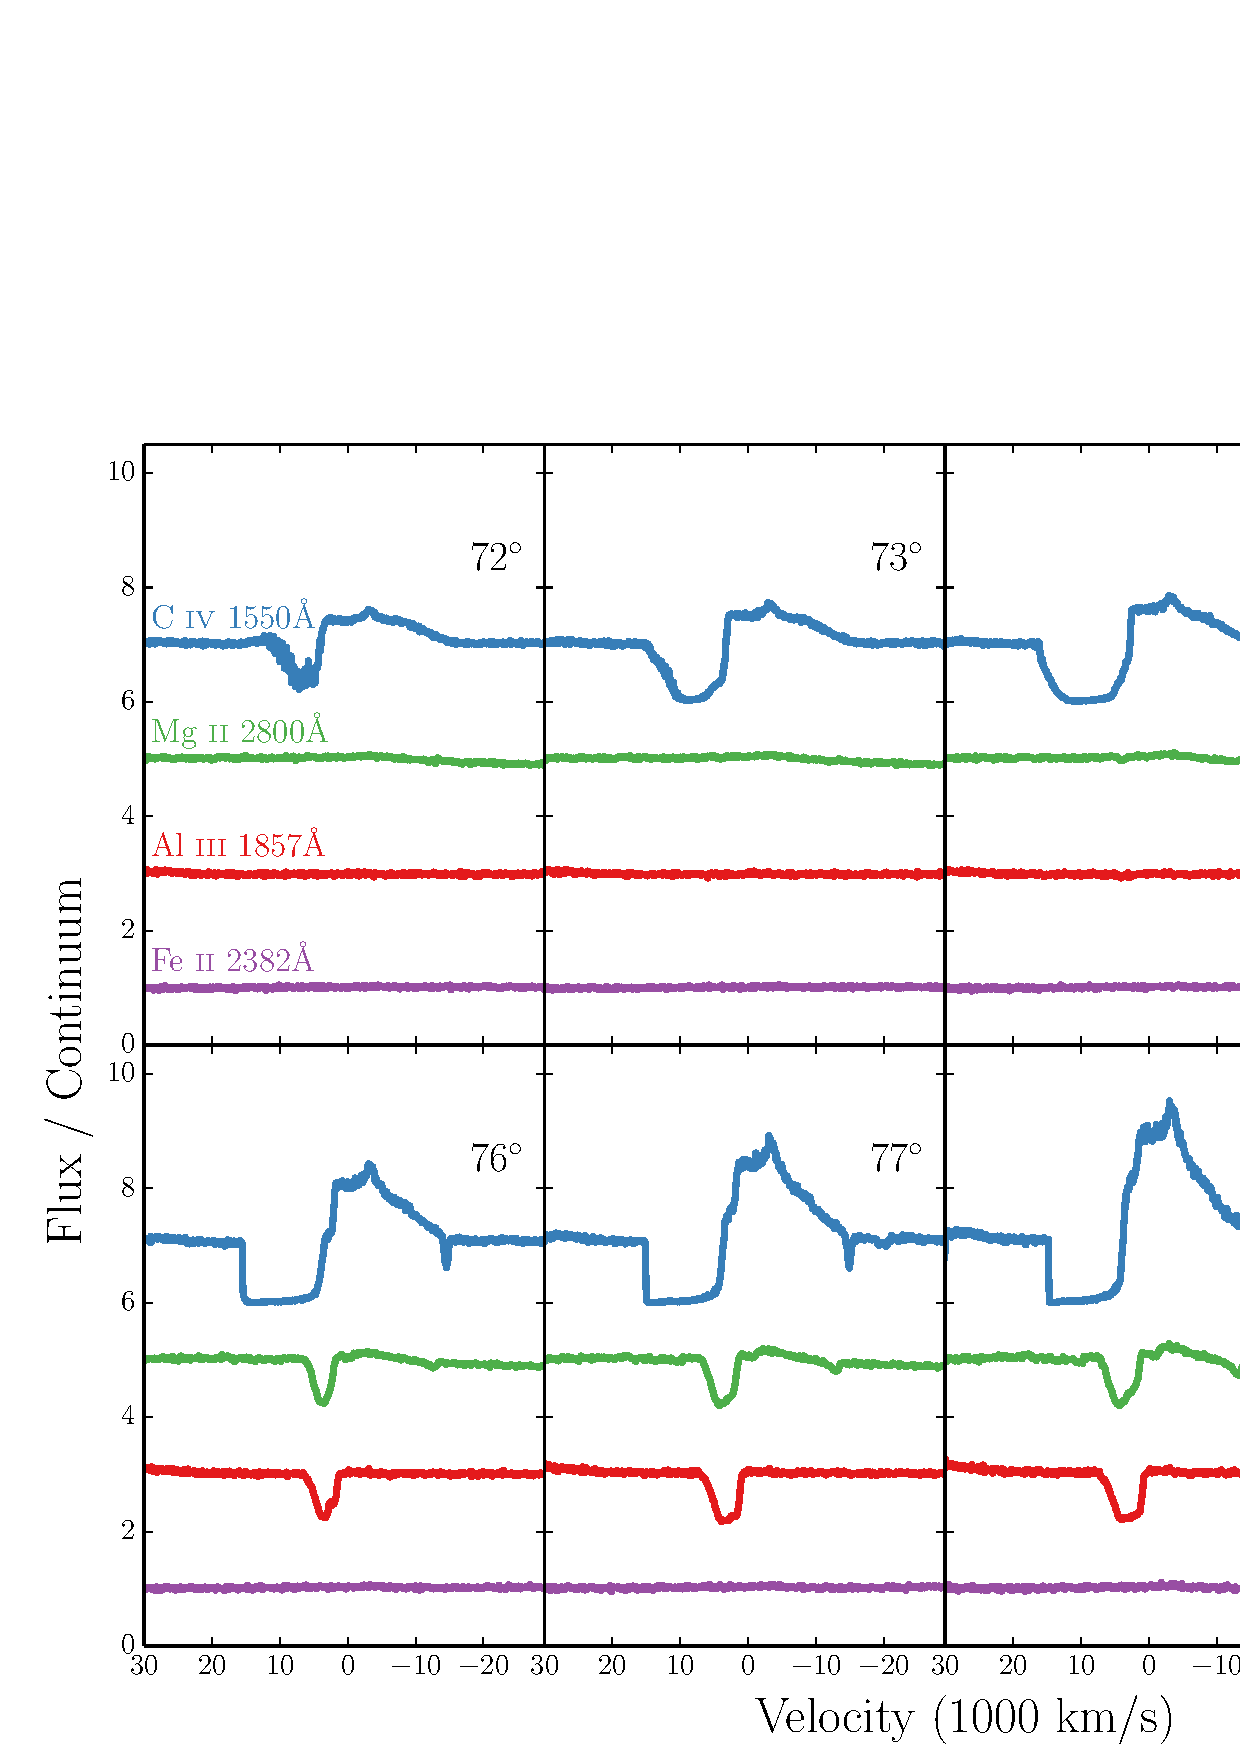
\includegraphics[width=1.0\textwidth]{figures/c4_angles.png}
\caption
{
\civ , \mg , \al\ and Fe~\textsc{ii} line profiles for viewing angles
from $72-79^\circ$. The profiles are plotted relative to the local
continuum with an offset applied for clarity. Lower ionization
profiles appear at a subset of high inclinations, compared
to the ubiquitous \civ\ profile.
}
\label{fig:lobal}
\end{figure*} %fullpage


At certain sightlines, the synthetic spectra exhibit blue-shifted BALs in \al\ and \mg --
the absorption lines seen in LoBALQSOs, and we even see absorption in Fe~\textsc{ii}
at the highest inclinations. Line profiles in velocity space 
for \civ, \al\ and \mg, are shown in figure~\ref{fig:lobal} for a range
of BALQSO viewing angles. We find that ionization stratification
of the wind causes lower ionization material to have a smaller covering factor, 
as demonstrated by figures~\ref{fig:wind} and \ref{fig:lobal}.
This confirms the behaviour expected from a unification model such as Elvis (2000). 
LoBALs are only present at viewing angles close to edge-on ($i>75^\circ$),
as predicted by polarisation results \citep{brotherton1997}.
As observed in a BALQSO sample by \cite{filizak2014}, we find that
BAL troughs are wider and deeper when low ionization absorption features are present,
and high ionization lines have higher blue-edge velocities than the 
low ionization species.
There is also a correlation between the strength of LoBAL features
and the amount of continuum attenuation at that sightline, particularly
blueward of the Lyman edge as the low ionization base 
intersects the line-of-sight. 
A model such as this therefore predicts that LoBALQSOs and FeLoBALQSOs 
have stronger Lyman edge absorption and 
are more Compton-thick than HiBALQSOs and Type 1 quasars.
An edge-on scenario also offers a potential explanation for the rarity of LoBAL and
FeLoBAL quasars, due to a foreshortened and attenuated continuum, 
although, as noted in section~\ref{discsed}, BAL fraction 
inferences are fraught with complex selection effects.


%%%%%%%%%%%%%%%%%%%%%%%%%%%%%%%%%%%%%%%%%%%%%%%%%

% SUMMARY

%%%%%%%%%%%%%%%%%%%%%%%%%%%%%%%%%%%%%%%%%%%%%%%%%

\section{Summary}

We have carried out MCRT simulations using a simple
prescription for a biconical disc wind, with
the aim of expanding on the work of H13 and assessing 
the viability of such a model for geometric unification of quasars.
We find the following main points:

\begin{enumerate}
\item We have introduced a first-order treatment 
of clumping in our model, and found that it can now maintain
the required ionization state while agreeing well with the X-ray
properties of AGN/QSOs.
\smallskip
\item We have shown that the degree of ionization stratification
in the model is sufficient that LoBAL line profiles
are seen at a subset of viewing angles, and Fe~\textsc{ii}
absorption is seen at particularly high inclinations.
\smallskip
\item We find that clumping also causes a significant 
increase in the strength of the  emission
lines produced by the model. This is true both
of collisionally excited resonance lines (such as \civ, \nv)
and recombination lines (such as \la, \ha\ and the Balmer series).
\smallskip
\item The line EWs in our models increase with inclination.
BAL and non-BAL quasar composites have comparable EWs, so our model
fails to reproduce this behaviour.
This is due to a fundamental constraint discussed further in section~\ref{sec:angular}. If the BLR
emits fairly isotropically then for a foreshortened, limb-darkened classical thin accretion disc
it is simply not possible to achieve line ratios at low inclinations that are comparable to
those at high inclinations. This is a robust conclusion which 
is independent of the assumed BLR geometry and size.
\end{enumerate}
Our work confirms a number of expected outcomes from a geometric unification 
model, and suggests that a simple biconical geometry such as this can come close to 
explaining much of the  phenomenology of quasars. Nevertheless, our conclusions pose 
a clear challenge to the current disc wind unification picture.

\section*{Acknowledgements}

The work of JHM, SWM, NSH and CK is supported by the
Science and Technology Facilities Council (STFC),
via two studentships and a consolidated grant, respectively.
CK also acknowledges a Leverhulme fellowship.
We would like to thank Omer Blaes, Ivan Hubeny and Shane Davis for their
assistance with \agn. We are grateful to Mike Brotherton, Mike DiPompeo,
Sebastien Hoenig and Frederic Marin for helpful correspondence regarding
polarisation measurements and orientation indicators.
We would also like to thank Daniel Proga, Daniel Capellupo, Sam Connolly and
Dirk Grupe for useful discussions.  Simulations were conducted using \py\ version 80,
and made use of the IRIDIS High Performance Computing Facility at the
University of Southampton. Figures were produced using the {\tt matplotlib} plotting library
\citep{matplotlib}.


%% \texttt{mn2e.cls} \textsc{Latex} document class. 

\bibliography{mybib.bib,stellar.bib,h14.bib,h13.bib,hamann.bib,krolik.bib}
\clearpage
\clearpage
%\appendix
% \appendix
% \section{Notes}


\end{document}
